% ==========================================
% LatexRefinement Step Output: step4-05-12-25-tuesday-all-offset-final.tex
% Model: gemini-3.5-flash
% Temperature: 0.36
% TopP: 0.95
% TopK: 40
% MaxOutputTokens: 65535
% ThinkingBudget: 32765
% ThinkingLevel: HIGH
% Prompt Tokens: 33'701
% Candidates Tokens: 18'728 (inkl. Thinking Tokens)
% Cached Tokens: 0
% Processed on: 2026-07-11 01:01:27
% ==========================================

% Primary Language: German

\lecturechapter{Dienstag}{12. Mai}{12. Mai 2026}{Der euklidische Algorithmus}

\begin{nice-box}[Kontext \& Agenda]
In diesem Kapitel beschäftigen wir uns mit der elementaren Zahlentheorie innerhalb der ganzen Zahlen $\mathbb{Z}$. Diese Konzepte bilden das Fundament für viele weiterführende Themen der Algebra und Kryptographie.

\textbf{Agenda:}
\begin{enumerate}[label=\textbf{(\arabic*)}]
    \item \textbf{Grundlagen der Teilbarkeit:} Definitionen, Notation und die Division mit Rest.
    \item \textbf{Der größte gemeinsame Teiler (ggT):} Existenz, Eigenschaften und die Bézout-Identität.
    \item \textbf{Der euklidische Algorithmus:} Praktische und effiziente Berechnung des $\operatorname{ggT}$.
    \item \textbf{Primzahlen:} Das Lemma von Euklid, der Fundamentalsatz der Arithmetik und die Unendlichkeit der Primzahlen.
    \item \textbf{Einführung in die Kongruenzrechnung:} Die Eulersche $\varphi$-Funktion und Rechnen mit Restklassen.
\end{enumerate}
\end{nice-box}

\section{Grundlagen der Teilbarkeit}

\begin{spoken-clean}[00:00:00 - 00:02:15]
Hallo zusammen, wir fangen an. Wir gehen jetzt über zum nächsten Kapitel. Ich folge jetzt zwar der Kapitelstruktur im Skript, aber wir machen das hier ein bisschen anders oder kürzer als im Skript.

Wir machen jetzt diese und nächste Woche --- wahrscheinlich auch noch die übernächste --- noch ein wenig elementare Zahlentheorie. Aber wirklich sehr elementar; das ist keine sehr tiefgehende Zahlentheorie, aber doch so viel, wie man auf jeden Fall im ersten Jahr sehen sollte. Und einiges davon haben Sie wahrscheinlich auch bereits gesehen.

Im Skript steht da noch vieles zu diesen Kettenbrüchen --- das ist zwar ein interessantes Thema, insbesondere geht es um die Frage, wie man reelle Zahlen durch rationale Zahlen approximieren kann und was es da für Möglichkeiten gibt ---, aber wir machen jetzt wirklich nur das über die ganzen Zahlen. Wenn Sie das interessiert, sind Sie herzlich eingeladen, das noch durchzulesen, aber ja, wir machen es jetzt ganz elementar.
\end{spoken-clean}

\subsection{Notation und Grundlagen der Teilbarkeit}

\begin{spoken-clean}[00:02:15 - 00:04:40]
In der Zahlentheorie interessiert man sich für die ganzen Zahlen oder sogar für die natürlichen Zahlen. Und okay, wir machen jetzt die Notation in diesem... ich folge jetzt auch wieder dem Skript. In diesem Kapitel schreiben wir $\mathbb{N}$ für die natürlichen Zahlen. Das heißt, das ist $0, 1, 2, 3$ und so weiter. Der wichtige Punkt ist, dass hier die $0$ auch drin ist.

Wir hatten vorher einmal angenommen, dass das gleich $\omega$ ist. Nun, $\omega$ verwendet man in der Regel nur in der Logik oder wenn man von Kardinalitäten und Ähnlichem spricht. In der restlichen Mathematik spricht man von den natürlichen Zahlen. Und okay, oft verwendet man dieses Symbol --- oder früher hat man es oft verwendet. Das Problem mit dem $\mathbb{N}$ für die natürlichen Zahlen ist, dass nicht immer klar ist, was gemeint ist. Es ist vielleicht so --- ich weiß nicht ---, die Hälfte der Leute würde sagen, dass die $0$ nicht dazugehört, und die andere Hälfte sagt, dass die $0$ dazugehört.

Ich habe da keine starke Meinung, aber es gibt Leute mit sehr starken Meinungen dazu. \inlinemetanote{lacht} Ich mache es einfach so, wie es im Skript ist, dass die $0$ mit dabei ist. Das ist so... ja, ich bin nicht ganz sicher über die Geschichte. Ich glaube, irgendwann im letzten Jahrhundert hat mal ein Mathematiker in Frankreich die Idee gehabt, dass es eine gute Idee sei, die $0$ dazuzunehmen. Und dadurch, dass das sehr renommierte Mathematiker waren, hat sich das gewissermaßen durchgesetzt. Aber es gibt eben auch immer noch viele, die die $0$ nicht dazunehmen. Das hat jetzt zur Folge, dass man das Symbol eigentlich gar nicht mehr unkommentiert verwenden kann, weil nie ganz klar ist, was gemeint ist.

Wenn ich also ein Paper schreibe --- und viele Leute machen das so ---, schreibt man oft einfach $\mathbb{Z}_{>0}$ oder $\mathbb{Z}_{\ge 0}$, denn dann ist direkt klar, was gemeint ist. Man muss nicht erst definieren, dass $\mathbb{N}$ dieses oder jenes ist; denn wenn man irgendeinen Satz aus der Mitte des Papers anschaut, ist sonst nicht klar, was gemeint ist. Okay, das Symbol ist also eigentlich fast zerstört in der heutigen Mathematik, eben weil es nicht mehr eindeutig definiert ist.
\end{spoken-clean}

\begin{math-stroke}[Notation der Zahlbereiche]
In diesem Kapitel verwenden wir folgende Konventionen:
\begin{itemize}
    \item \textbf{Natürliche Zahlen:} $\mathbb{N} = \{0, 1, 2, 3, \dots\} = \omega$.
    \item \textbf{Ganze Zahlen:} $\mathbb{Z} = \{\dots, -2, -1, 0, 1, 2, \dots\}$.
\end{itemize}

\begin{remark}[Notation der natürlichen Zahlen]
Die Inklusion der Null in $\mathbb{N}$ wird in der Literatur uneinheitlich gehandhabt. Zur Vermeidung von Ambiguitäten empfiehlt sich in wissenschaftlichen Publikationen die explizite Notation $\mathbb{Z}_{>0}$ bzw. $\mathbb{Z}_{\ge 0}$.
\end{remark}
\end{math-stroke}

\begin{spoken-clean}[00:04:40 - 00:07:10]
Gut. Okay, jetzt eine ganz einfache Definition. Wir schauen uns jetzt ganze Zahlen an. Seien $a, b$ ganze Zahlen. Dann sagen wir, dass $a$ die Zahl $b$ teilt --- oder $b$ ein Vielfaches von $a$ ist ---, falls ein $c$ existiert, sodass $b = a \cdot c$ ist. Und wir verwenden als Notation, weil wir das so oft schreiben, einfach $a \mid b$. Haben Sie bestimmt auch schon gesehen.

Und das ist das Schöne an den ganzen Zahlen --- das, was die ganzen Zahlen überhaupt so spannend macht ---: dass gewisse Zahlen einander teilen und andere nicht. Das hat man in einem Körper ja nicht. In einem Körper teilt alles alles, solange es nicht null ist. Das ist das Schöne an einem Körper --- beziehungsweise ist ein Körper aus anderen Gründen schön ---, aber das hier macht die ganzen Zahlen eben sehr interessant. Und wie Sie wissen, führt das alles sehr, sehr schnell zu äußerst schwierigen Fragen, die sehr tief gehen und die man bis heute noch nicht ganz versteht.
\end{spoken-clean}

\begin{math-stroke}[Teilbarkeit in den ganzen Zahlen]
\begin{definition}[Teilbarkeit]\label[definition]{def:teilbarkeit}
Seien $a, b \in \mathbb{Z}$. Wir sagen, \newterm{$a$ teilt $b$} (geschrieben $a \mid b$), falls ein $c \in \mathbb{Z}$ existiert, sodass gilt:
\[
b = a \cdot c.
\]
In diesem Fall nennen wir $b$ auch ein \newterm{Vielfaches} von $a$.
\end{definition}
\end{math-stroke}

\begin{didactic-insight}[Teilbarkeit: Ringe vs. Körper]
In einem Körper (wie $\mathbb{R}$ oder $\mathbb{Q}$) ist die Teilbarkeit trivial, da jedes Element $a \neq 0$ ein inverses Element $a^{-1}$ besitzt und somit $b = a \cdot (a^{-1}b)$ für alle $b$ gilt. Die Struktur der ganzen Zahlen $\mathbb{Z}$ als Ring (ohne multiplikative Inverse für alle Elemente außer $1$ und $-1$) macht den Begriff der Teilbarkeit erst mathematisch gehaltvoll und führt zur Primzahltheorie.
\end{didactic-insight}

\subsection{Division mit Rest}

\begin{spoken-clean}[00:07:10 - 00:08:30]
Gut. Machen wir als Nächstes eine einfache Proposition oder ein Lemma: das Teilen mit Rest. Sehr nützlich! Sei $a$ eine natürliche Zahl und $b$ irgendeine ganze Zahl. Dann existieren eindeutige ganze Zahlen $q$ und $r$, sodass wir $b = a \cdot q + r$ haben, wobei dieses $r$ größer gleich null, aber strikt kleiner als $a$ ist.

Okay, das ist genau das, was Sie schon in der Grundschule machen: Teilen mit Rest. Man schaut, wie oft $a$ in $b$ hineinpasst, und dann bleibt eben noch ein Rest übrig, der aber strikt kleiner ist als $a$. Das ist relativ zentral, und dass man das in den ganzen Zahlen so machen kann, ist eine sehr schöne Eigenschaft.

Der Beweis ist sehr direkt. Wir schreiben das jetzt ein bisschen hochgestochener auf, als man es eigentlich müsste. Wir betrachten die Menge $S$ aller Zahlen der Form $b - a \cdot s$, wobei $s$ eine beliebige Zahl in $\mathbb{Z}$ ist, und wir nehmen nur diejenigen davon, die größer gleich null sind. Aus dieser Menge wählen wir das kleinste Element --- also das Minimum. Das geht, weil wir uns in den natürlichen Zahlen befinden, und diese sind bekanntlich wohlgeordnet.
\end{spoken-clean}

\begin{math-stroke}[Division mit Rest]
\begin{proposition}[Teilen mit Rest]\label[proposition]{prop:teilen-mit-rest}
Sei $a \in \mathbb{N} \setminus \{0\}$ und $b \in \mathbb{Z}$. Dann existieren eindeutig bestimmte Zahlen $q, r \in \mathbb{Z}$, sodass gilt:
\begin{equation}\label{eq:division-rest}
b = a \cdot q + r \quad \text{mit} \quad 0 \le r < a.
\end{equation}
Hierbei heißt $q$ der \newterm{Quotient} und $r$ der \newterm{Rest}.
\end{proposition}
\end{math-stroke}

\begin{proof}[Beweis von Proposition \ref{prop:teilen-mit-rest}]
\begin{spoken-clean}[00:08:30 - 00:11:00]
Und okay, wenn wir so ein $r$ haben, nehmen wir noch ein $q \in \mathbb{Z}$ hinzu, sodass wir $b - a \cdot q = r$ schreiben können. Genau. Und dieses $r$ ist ja größer gleich null, da wir die Menge mit den nicht-negativen ganzen Zahlen geschnitten haben.

Jetzt zeigen wir zuerst, dass $r$ strikt kleiner ist als $a$. Das ist für dieses minimale Element sehr direkt. Denn wäre $r \ge a$ --- falls das also nicht der Fall ist ---, dann betrachten wir $b - a \cdot (q + 1)$. Das ist dasselbe wie $b - aq - a$, was wiederum gleich $r - a$ ist. Wenn nun $r \ge a$ wäre, dann wäre dieser Ausdruck ebenfalls wieder größer gleich null. Da wir aber angenommen hatten, dass $r$ das minimale Element in $S$ ist, stünde dies im Widerspruch zur Minimalität von $r$ in $S$.

Das heißt, $r$ muss kleiner als $a$ sein. Und dann müssen wir noch zeigen, dass diese Zahlen eindeutig sind. Dazu nehmen wir an, dass es zwei solche Darstellungen gibt. Wir können also schreiben: $b = a \cdot q_1 + r_1$, und das soll dasselbe sein wie $a \cdot q_2 + r_2$.
\end{spoken-clean}

\begin{math-stroke}[Beweis der Existenz und Schranke für den Rest]
\begin{short-proof}[Beweis der Existenz]
Wir definieren die Menge $S$ aller nicht-negativen Reste:
\[
S := \{ b - a \cdot s \mid s \in \mathbb{Z} \} \cap \mathbb{N}.
\]
\textbf{1. $S$ ist nicht leer:} 
Da $a \ge 1$, können wir $s$ so wählen, dass $a \cdot s$ sehr klein (negativ) wird, wodurch $b - as$ positiv wird. Somit ist $S \neq \emptyset$.

\textbf{2. Wahl des minimalen Elements:}
Da $S$ eine nichtleere Teilmenge der natürlichen Zahlen $\mathbb{N}$ ist, besitzt sie nach dem \newterm{Wohlordnungsprinzip} ein minimales Element. Wir setzen:
\[
r := \min(S).
\]
Da $r \in S$, existiert ein $q \in \mathbb{Z}$, sodass $r = b - a \cdot q$, also $b = a \cdot q + r$. Nach Konstruktion gilt $r \ge 0$.
\end{short-proof}

\begin{short-proof}[Nachweis von $r < a$]
Angenommen, es wäre $r \ge a$. Wir betrachten das Element:
\begin{align*}
r' &:= b - a \cdot (q + 1) \\
&= (b - a \cdot q) - a \\
&= r - a.
\end{align*}
Da $r \ge a$, gilt $r' = r - a \ge 0$, folglich ist $r' \in S$. Da jedoch $a > 0$, gilt $r' < r$. Dies steht im Widerspruch zur Minimalität von $r$ in $S$. Also muss $r < a$ gelten.
\end{short-proof}
\end{math-stroke}

\begin{spoken-clean}[00:11:00 - 00:12:20]
Daraus folgt natürlich, wenn die beiden Ausdrücke gleich sind: $r_1 - r_2$ ist dasselbe wie $a \cdot (q_2 - q_1)$. Okay, aber $a$ ist ja positiv. Falls wir nun annehmen, dass $q_1 \neq q_2$ ist, dann würde folgen, dass $a \cdot |q_2 - q_1|$ größer gleich $a$ sein muss.
\end{spoken-clean}

\begin{spoken-clean}[00:12:20 - 00:13:40]
Aber die Differenz der Reste im Betrag ist ja strikt kleiner als $a$. Das ist ein Widerspruch dazu, dass $|r_1 - r_2| < a$ gelten muss.

Das heißt also, diese Annahme ist nicht möglich. Daraus erhalten wir $q_1 = q_2$ und somit auch $r_1 = r_2$. Okay, das ist relativ direkt.

Soweit alles klar? Die Aussage ist ja eigentlich auch schon anschaulich klar, wenn man sie so aufschreibt. Das weiß man wie gesagt schon aus der Grundschule, dass das Teilen mit Rest eindeutig ist. Das ist also keine große Überraschung, oder?
\end{spoken-clean}

\begin{math-stroke}[Fortsetzung des Beweises: Eindeutigkeit]
\begin{short-proof}[Beweis der Eindeutigkeit]
Angenommen, es gäbe zwei Darstellungen:
\[
b = a \cdot q_1 + r_1 = a \cdot q_2 + r_2 \quad \text{mit} \quad 0 \le r_1, r_2 < a.
\]
Durch Umstellen erhalten wir:
\begin{equation}\label{eq:eindeutigkeit-differenz}
r_1 - r_2 = a \cdot (q_2 - q_1).
\end{equation}
Wir betrachten die Beträge: $|r_1 - r_2| = a \cdot |q_2 - q_1|$.
Da $0 \le r_1, r_2 < a$, gilt für die Differenz:
\[
-a < r_1 - r_2 < a \implies |r_1 - r_2| < a.
\]
Wäre $q_1 \neq q_2$, so wäre $|q_2 - q_1| \ge 1$. Da $a \ge 1$, folgte:
\[
|r_1 - r_2| = a \cdot |q_2 - q_1| \ge a \cdot 1 = a.
\]
Dies widerspricht $|r_1 - r_2| < a$. Folglich muss $q_1 = q_2$ gelten. Aus \eqref{eq:eindeutigkeit-differenz} folgt dann unmittelbar $r_1 - r_2 = 0$, also $r_1 = r_2$.
\end{short-proof}
\end{math-stroke}
\end{proof}

\begin{student-interaction}[Studentenfrage]
Was ist, wenn $a = 0$ ist? Ich glaube, bestimmte Argumente funktionieren dann nicht mehr, zum Beispiel wenn wir zeigen, dass $r$ strikt kleiner ist als $a$, obwohl wir explizit angenommen haben, dass $r$ nicht negativ ist. Die Proposition gilt dann trotzdem, aber...
\end{student-interaction}

\begin{spoken-clean}[00:13:40 - 00:15:20]
Ah, nein, dann ist $q$ nicht mehr eindeutig --- ja, natürlich! Wenn $a = 0$ ist, ist $q$ nicht mehr eindeutig, da haben Sie völlig recht. Wir müssen also voraussetzen, dass $a$ nicht null sein darf. Wenn $a$ null wäre, dann würden wir hier etwas Widersprüchliches beweisen. Das geht natürlich nicht; $a$ kann nicht null sein. Ja, gute Bemerkung! Genau, das ist das Problem.

Schreiben wir also $a \neq 0$ hin, ich glaube, das ist besser. Wenn $a$ null ist... ja, dann kann man... ja, schließen wir den Fall $a = 0$ einfach aus, sonst funktioniert es nicht. Das macht sonst wenig Sinn. Danke!
\end{spoken-clean}

\begin{meta-note}[Korrektur an der Tafel]
Der Dozent korrigiert die Voraussetzung in der Proposition an der Tafel von $a \in \mathbb{N}$ zu $a \in \mathbb{N} \setminus \{0\}$.
\end{meta-note}

\begin{math-stroke}[Korrektur der Voraussetzung]
In Proposition \ref{prop:teilen-mit-rest} muss zwingend $a \neq 0$ gelten, damit der Quotient $q$ eindeutig bestimmt ist. Falls $a = 0$, wäre $b = 0 \cdot q + r = r$, wodurch $r = b$ feststünde, aber $q$ beliebig gewählt werden könnte. Zudem wäre die Bedingung $0 \le r < 0$ für $b \neq 0$ unmöglich zu erfüllen.
\end{math-stroke}

\subsection{Der größte gemeinsame Teiler (ggT)}

\begin{spoken-clean}[00:15:20 - 00:17:50]
Okay. Dann machen wir als Nächstes weiter mit dem größten gemeinsamen Teiler. Das ist die nächste Proposition, die Sie vielleicht auch schon einmal gesehen haben. Wir nehmen zwei natürliche Zahlen $a, b$, und diesmal nehmen wir an, dass sie nicht beide null sind --- um ganz sicherzugehen. Dann existiert ein eindeutiges $d \in \mathbb{N}$, sodass gilt: $d$ teilt $a$ und $d$ teilt $b$.

Und das Zweite ist: Für alle natürlichen Zahlen $k$, die sowohl $a$ als auch $b$ teilen, gilt, dass $k$ auch $d$ teilt. Das heißt, $d$ wird von allen anderen gemeinsamen Teilern geteilt. Okay, und außerdem existieren ganze Zahlen $x$ und $y$ in $\mathbb{Z}$, sodass $d = a \cdot x + b \cdot y$ gilt. Also lässt sich $d$ als eine Linearkombination von $a$ und $b$ darstellen.

\inlinemetanote{korrigiert sich an der Tafel} $k$ teilt $d$, oder? Wir wollen ja den größten gemeinsamen Teiler, nicht das kleinste gemeinsame Vielfache. Genau! Dieses $d$ heißt der größte gemeinsame Teiler von $a$ und $b$. Auch dieser Begriff ist Ihnen bestimmt schon einmal begegnet --- vielleicht irgendwann in der Schule ---: Es ist einfach die größte natürliche Zahl, die beide Zahlen teilt.
\end{spoken-clean}

\begin{math-stroke}[Der größte gemeinsame Teiler]
\begin{proposition}[Existenz und Eigenschaften des ggT]\label[proposition]{prop:ggt-existenz}
Seien $a, b \in \mathbb{N}$, wobei nicht beide null sind. Dann existiert eine eindeutig bestimmte Zahl $d \in \mathbb{N} \setminus \{0\}$ mit folgenden Eigenschaften:
\begin{enumerate}[label=\textbf{(\alph*)}]
    \item $d \mid a$ und $d \mid b$ ($d$ ist ein gemeinsamer Teiler).
    \item Für jedes $k \in \mathbb{N}$ gilt: Falls $k \mid a$ und $k \mid b$, dann folgt $k \mid d$ ($d$ wird von jedem gemeinsamen Teiler geteilt).
\end{enumerate}
Zudem existieren $x, y \in \mathbb{Z}$, sodass gilt:
\begin{equation}\label{eq:bezout-identitaet}
d = a \cdot x + b \cdot y \quad (\text{\newterm{Bézout-Identität}}).
\end{equation}
\end{proposition}

\begin{definition}[Größter gemeinsamer Teiler]\label[definition]{def:ggt}
Die Zahl $d$ aus Proposition \ref{prop:ggt-existenz} heißt der \newterm{größte gemeinsame Teiler} von $a$ und $b$. Wir schreiben:
\[
d = \operatorname{ggT}(a, b) \quad (\text{englisch: } \operatorname{gcd}(a, b) \text{ für \emph{greatest common divisor}}).
\]
\end{definition}
\end{math-stroke}

\begin{proof}[Beweis von Proposition \ref{prop:ggt-existenz}]
\begin{spoken-clean}[00:17:50 - 00:20:15]
Für den Beweis betrachten wir wieder eine geeignete Menge, aus der wir das minimale Element wählen. Dazu definieren wir $I$ als die Menge aller ganzzahligen Linearkombinationen der Form $a \cdot u + b \cdot v$, wobei $u, v \in \mathbb{Z}$ sind, und wir betrachten nur die positiven Elemente daraus.

Aus dieser Menge nehmen wir nun das minimale Element. Sei $d \in I$ minimal. Dann existieren $x, y \in \mathbb{Z}$, sodass wir $d = a \cdot x + b \cdot y$ schreiben können. Wir betrachten also per Definition alle positiven Linearkombinationen dieser Form und wählen davon die kleinste. Genau. Wenn wir nun zeigen, dass dieses $d$ die Eigenschaften \textbf{(a)} und \textbf{(b)} erfüllt, dann erhalten wir diese Darstellung als Linearkombination quasi gratis dazu.
\end{spoken-clean}

\begin{math-stroke}[Beweis der Existenz des ggT]
\begin{short-proof}[Beweis der Existenz]
Wir betrachten die Menge aller positiven ganzzahligen Linearkombinationen von $a$ und $b$:
\[
I := \{ a \cdot u + b \cdot v \mid u, v \in \mathbb{Z} \} \cap \mathbb{Z}_{>0}.
\]
\textbf{1. $I$ ist nicht leer:}
Da $a, b$ nicht beide null sind, ist mindestens eines der Elemente $a, b, -a, -b$ in $I$ enthalten.

\textbf{2. Wahl des minimalen Elements:}
Nach dem Wohlordnungsprinzip existiert ein minimales Element $d \in I$. Da $d \in I$, existieren $x, y \in \mathbb{Z}$, sodass:
\[
d = a \cdot x + b \cdot y.
\]
Wir zeigen nun, dass dieses $d$ die Eigenschaften \textbf{(a)} und \textbf{(b)} erfüllt.
\end{short-proof}
\end{math-stroke}

\begin{spoken-clean}[00:20:15 - 00:22:45]
Die Behauptung, die wir nun beweisen wollen, ist, dass $d$ jedes Element in dieser Menge $I$ teilt. Daraus folgt dann auch direkt der Rest der Proposition. Sei also $z = a \cdot u + b \cdot v$ für beliebige ganze Zahlen $u$ und $v$. Dann gilt, dass $d$ ein Teiler von $z$ ist.

Der Beweis dieser Behauptung läuft wie folgt: Wir führen eine Division mit Rest durch und schreiben $z = d \cdot q + r$ mit $0 \le r < d$. In solchen Situationen ist die Division mit Rest eigentlich immer die beste Idee. Da $d$ minimal gewählt war, können wir nämlich zeigen, dass dieser Rest $r$ zwingend null sein muss.

Wir können nämlich schreiben: $r = z - d \cdot q$. Da wir wissen, dass sowohl $z$ als auch $d$ von dieser Form sind, muss auch $r$ wieder eine solche Linearkombination sein. Das heißt, wir können schreiben: $r = a \cdot (u - q \cdot x) + b \cdot (v - q \cdot y)$.

Nun gilt nach Voraussetzung $r \ge 0$. Da wir aber angenommen hatten, dass $d$ das minimale positive Element mit dieser Eigenschaft ist, muss $r$ zwingend null sein --- denn es kann kein strikt kleines positives Element in $I$ geben. Also ist $r = 0$, woraus folgt, dass $z$ ein Vielfaches von $d$ ist. Das heißt, $d$ teilt $z$. Okay, das ist relativ direkt.
\end{spoken-clean}

\begin{math-stroke}[Nachweis der Teilereigenschaft]
\begin{claim}
Das minimale Element $d \in I$ teilt jedes Element $z \in \{ a \cdot u + b \cdot v \mid u, v \in \mathbb{Z} \}$.
\end{claim}

\begin{short-proof}
Sei $z = a \cdot u + b \cdot v$ beliebig. Wir führen eine Division von $z$ durch $d$ mit Rest durch:
\[
z = d \cdot q + r \quad \text{mit} \quad 0 \le r < d.
\]
Wir stellen nach $r$ um:
\begin{align*}
r &= z - d \cdot q \\
&= (a \cdot u + b \cdot v) - (a \cdot x + b \cdot y) \cdot q \\
&= a \cdot (u - qx) + b \cdot (v - qy).
\end{align*}
Somit ist $r$ ebenfalls eine ganzzahlige Linearkombination von $a$ und $b$. 
Wäre $r > 0$, so wäre $r \in I$. Da aber $r < d$, stünde dies im Widerspruch zur Minimalität von $d$ in $I$. 
Folglich muss $r = 0$ gelten. Daraus folgt $z = d \cdot q$, also $d \mid z$.
\end{short-proof}

\begin{explanation-of-steps}[Abschluss des Beweises von Proposition \ref{prop:ggt-existenz}]
\begin{itemize}
    \item \textbf{Eigenschaft (a):} Da $a = a \cdot 1 + b \cdot 0$ und $b = a \cdot 0 + b \cdot 1$ Linearkombinationen sind, folgt aus dem Claim sofort $d \mid a$ und $d \mid b$.
    \item \textbf{Eigenschaft (b):} Sei $k$ ein gemeinsamer Teiler von $a$ und $b$. Dann gilt $a = m \cdot k$ und $b = n \cdot k$. Einsetzen in die Bézout-Identität liefert:
    \[ d = (mk) \cdot x + (nk) \cdot y = k \cdot (mx + ny) \implies k \mid d. \]
\end{itemize}
\end{explanation-of-steps}
\end{math-stroke}

\begin{spoken-clean}[00:22:45 - 00:24:50]
Aus dieser Behauptung können wir nun die Proposition ableiten. Die Behauptung haben wir damit bewiesen. Und wir sehen: Aus der Behauptung folgt direkt Eigenschaft \textbf{(a)}, da sowohl $a$ als auch $b$ von dieser Form sind. Die Behauptung impliziert also \textbf{(a)}.

Es bleibt uns noch, Eigenschaft \textbf{(b)} zu beweisen. Für \textbf{(b)}: Falls $k$ ein Teiler von $a$ und $k$ auch ein Teiler von $b$ ist, dann können wir schreiben: $d = m \cdot k \cdot x + n \cdot k \cdot y$. Das ist dasselbe wie $k \cdot (mx + ny)$. Klar: Wenn $k$ die beiden Summanden teilt, dann teilt es auch deren Summe. Das heißt, $d$ ist ein Vielfaches von $k$. Genau das beweist \textbf{(b)}.

Schließlich können wir noch sehen, dass $d$ eindeutig ist. Falls ein $d' \in \mathbb{N}$ sowohl \textbf{(a)} als auch \textbf{(b)} erfüllt, so folgt, dass $d$ die Zahl $d'$ teilt und $d'$ wiederum $d$ teilt. Das folgt direkt aus Eigenschaft \textbf{(b)}. Wenn zwei natürliche Zahlen sich gegenseitig teilen, dann bedeutet das: $d = u \cdot d'$ und $d' = v \cdot d$ für gewisse ganze Zahlen $u$ und $v$. Daraus folgt $d = u \cdot v \cdot d$, was bedeutet, dass $u \cdot v = 1$ sein muss. Da wir uns in den natürlichen Zahlen befinden und $d \neq 0$ ist, folgt daraus direkt $d = d'$. Genau, da $d$ nicht null ist, weil wir ja vorausgesetzt haben, dass die beiden Ausgangszahlen nicht beide null sind. \inlinemetanote{lacht} Ob ich sonst noch eine Null vergessen habe... nein, ich glaube, jetzt sollte es funktionieren.
\end{spoken-clean}

\begin{math-stroke}[Eindeutigkeit des ggT]
\begin{short-proof}[Beweis der Eindeutigkeit]
Angenommen, es gäbe zwei Zahlen $d, d' \in \mathbb{N}$, die beide die Eigenschaften \textbf{(a)} und \textbf{(b)} erfüllen.
\begin{itemize}
    \item Da $d$ ein gemeinsamer Teiler ist und $d'$ die Eigenschaft \textbf{(b)} erfüllt, folgt $d \mid d'$.
    \item Da $d'$ ein gemeinsamer Teiler ist und $d$ die Eigenschaft \textbf{(b)} erfüllt, folgt $d' \mid d$.
\end{itemize}
Aus $d \mid d'$ und $d' \mid d$ folgt für natürliche Zahlen unmittelbar $d = d'$.
\end{short-proof}
\end{math-stroke}
\end{proof}

\begin{student-interaction}[Studentenfrage]
Haben Sie am Anfang nicht gesagt, das kleinste gemeinsame Vielfache? Was, wenn beide null sind? Das Problem ist, wenn beide null sind, dann teilen alle Zahlen die Null.
\end{student-interaction}

\begin{spoken-clean}[00:24:50 - 00:26:41]
Ah ja, dann hat man einfach... die Zahl, die nicht null ist, ist dann der $\operatorname{ggT}$. Also so wie ich die Menge definiert habe, sind $a$ und $b$ ja generell auch in $I$ enthalten, das ist so, ja. Aber wenn $d$ minimal sein soll... genau, absolut! Aber $a$ und $b$ sind ja nicht... nein, das kann man so nicht sagen. \inlinemetanote{lacht} Weil sonst könnte man sie voneinander subtrahieren und dann... Wenn $a = 2$ and $b = 3$ ist, ja genau, dann ist $d = 1$. $2$ ist in der Menge drin, $3$ ist auch drin, aber keines davon ist minimal. Da hat man zum Beispiel $3 - 2$, das ist dann auch drin und das ist $1$.
\end{spoken-clean}

\begin{student-interaction}[Studentenfrage]
Was passiert im Fall $a = b = 0$?
\end{student-interaction}

\begin{math-stroke}[Ergänzung zum Existenzbeweis des ggT]
\begin{explanation-of-steps}
Falls $a = b = 0$, so ist jede ganze Zahl $k \in \mathbb{Z} \setminus \{0\}$ ein gemeinsamer Teiler, da $k \mid 0$ für alle $k$ gilt. In diesem Fall existiert kein \emph{größter} gemeinsamer Teiler im Sinne einer maximalen Zahl. Deshalb setzen wir in Proposition \ref{prop:ggt-existenz} voraus, dass $a$ und $b$ nicht beide null sind.

In der Menge $I = \{ au + bv \mid u, v \in \mathbb{Z} \} \cap \mathbb{Z}_{>0}$ sind für $a, b \neq 0$ stets positive Werte enthalten (z.\,B. $|a|$ oder $|b|$). Das minimale Element $d$ dieser Menge ist der $\operatorname{ggT}(a, b)$.
\end{explanation-of-steps}
\end{math-stroke}

\begin{spoken-clean}[00:26:41 - 00:28:29]
Das $I$ enthält also alle ganzzahligen Linearkombinationen. In Ihrem Beispiel ist $I$ die Menge aller $u \cdot 2 + 3 \cdot v$ mit $u, v \in \mathbb{Z}$, geschnitten mit den positiven ganzen Zahlen. Und das wäre jetzt zum Beispiel genau die Menge $\{1, 2, 3, \dots\}$. Okay? Wenn Sie $u = -1$ und $v = 1$ nehmen, dann haben Sie $2 \cdot (-1) + 3 \cdot 1 = 1$.

Der Fall, dass dieses $d$ genau die kleinere der beiden Zahlen ist --- vorausgesetzt, beide sind nicht null ---, entspricht genau dem Fall, in dem eine Zahl die andere teilt.

Wir werden gleich noch sehen, wie man diesen $\operatorname{ggT}$ berechnet --- das ist der euklidische Algorithmus. Das ist wirklich eine sehr schöne Sache. Sie kennen bestimmt von Euklid die \qt{Elemente} --- ein fantastisches Werk, das über 2000 Jahre alt und im Grunde immer noch aktuell ist. Klar, man hat heute etwas andere Vorstellungen von Axiomatik und so weiter, aber im Wesentlichen war das Buch absolut bahnbrechend. Dass es heute immer noch aktuell ist, zeigt die Beständigkeit der Mathematik, und es ist wirklich brillant, was er darin macht.

Wenn Sie also mal Zeit haben, ein bisschen in den \qt{Elementen} von Euklid zu lesen: Das ist sehr zu empfehlen. Es ist auch heute noch gut verständlich --- man muss sich natürlich ein bisschen in die historische Sprache einlesen, aber es ist wirklich ein sehr schönes Buch. Wir werden gleich sehen, wie man den $\operatorname{ggT}$ konkret berechnet. Aber zuerst machen wir eine kurze Pause.
\end{spoken-clean}

\begin{meta-note}[Vorlesungspause]
Der Dozent kündigt eine kurze Pause an, bevor er im nächsten Teil den euklidischen Algorithmus zur praktischen Berechnung des $\operatorname{ggT}$ erläutert.
\end{meta-note}

\section{Der euklidische Algorithmus}

\begin{meta-note}[Tafelübergang]
Der Dozent wischt die Tafel und bereitet die Einführung des euklidischen Algorithmus vor.
\end{meta-note}

\begin{spoken-clean}[00:28:29 - 00:29:45]
Gut, dann schauen wir uns das an. Wir haben zwei ganze Zahlen $a$ und $b$, und wir nehmen an, dass $a$ kleiner als $b$ ist. Wenn sie gleich sind, haben wir den $\operatorname{ggT}$ ja bereits direkt gegeben. Was wir nun eigentlich machen, ist, dass wir sukzessive mit Rest teilen.

Wir können schreiben... seien $q_1$ bis $q_{n+1}$ ganze Zahlen, und wir erhalten eine Kette von Resten, sodass gilt: $0 < r_n < r_{n-1} < \dots < r_1 < a$ gilt.
\end{spoken-clean}

\begin{spoken-clean}[00:29:45 - 00:31:04]
Sodass... wir schreiben das jetzt ein bisschen... so wie es hier aufgeschrieben ist, sieht es fast nach \qt{Reverse Engineering} aus.

Man macht im Grunde das Umgekehrte. Was man konkret tut, ist Folgendes: Man führt eine Division mit Rest durch. Wir teilen $b$ durch $a$ mit Rest und erhalten $b = a \cdot q_1 + r_1$. Als Nächstes teilen wir $a$ durch diesen ersten Rest $r_1$ --- ebenfalls wieder mit Rest. Wir schreiben also $a = r_1 \cdot q_2 + r_2$, was uns einen weiteren Rest $r_2$ liefert.
\end{spoken-clean}

\begin{math-stroke}[Der euklidische Algorithmus]
Seien $a, b \in \mathbb{N}$ mit $0 < a < b$. Der \newterm{euklidische Algorithmus} besteht aus einer Folge von Divisionen mit Rest:
\begin{align}
b &= a \cdot q_1 + r_1 && \text{mit } 0 \le r_1 < a \label{eq:euclid-step1} \\
a &= r_1 \cdot q_2 + r_2 && \text{mit } 0 \le r_2 < r_1 \label{eq:euclid-step2} \\
r_1 &= r_2 \cdot q_3 + r_3 && \text{mit } 0 \le r_3 < r_2 \label{eq:euclid-step3} \\
&\vdots \nonumber \\
r_{n-2} &= r_{n-1} \cdot q_n + r_n && \text{mit } 0 \le r_n < r_{n-1} \label{eq:euclid-step-n} \\
r_{n-1} &= r_n \cdot q_{n+1} + 0 \label{eq:euclid-step-final}
\end{align}

\begin{explanation-of-steps}
Da die Reste eine streng monoton fallende Folge natürlicher Zahlen bilden ($a > r_1 > r_2 > r_3 > \dots \ge 0$), muss der Algorithmus nach endlich vielen Schritten mit dem Rest $0$ terminieren.
\end{explanation-of-steps}
\end{math-stroke}

\begin{spoken-clean}[00:31:04 - 00:32:20]
Und dann teilen wir wieder... jetzt haben wir einfach die Rollen vertauscht: $a$ wird durch $r_1$ ersetzt, und wir teilen nun $r_1$ durch diesen neuen Rest $r_2$. Wir schreiben also $r_1 = r_2 \cdot q_3 + r_3$ plus einen weiteren Rest. Das machen wir immer so weiter, bis wir schließlich bei $r_{n-2}$ ankommen.
\end{spoken-clean}

\begin{spoken-clean}[00:32:20 - 00:33:39]
Das ist dann gleich $r_{n-1} \cdot q_n + r_n$.

Diese Reste werden natürlich immer kleiner: $r_1$ ist strikt kleiner als $a$, $r_2$ ist strikt kleiner als $r_1$, $r_3$ ist strikt kleiner als $r_2$ und so weiter. Sie bilden also eine streng monoton fallende Folge natürlicher Zahlen, die nach unten durch Null beschränkt ist. Das bedeutet, dass dieser Prozess irgendwann abbrechen muss; er kann nicht unendlich weitergehen. Irgendwann geht die Division also auf, und wir erhalten $r_{n-1} = r_n \cdot q_{n+1}$ ohne Rest.

Der euklidische Algorithmus besteht nun einfach darin, dass man diese Division mit Rest so lange wiederholt, bis der Rest null ist. Die Behauptung ist, dass der $\operatorname{ggT}$ von $a$ und $b$ genau dieser letzte von null verschiedene Rest $r_n$ ist.
\end{spoken-clean}

\begin{math-stroke}[Korrektheit des euklidischen Algorithmus]
\begin{proposition}\label[proposition]{prop:euclid-correctness}
Der letzte von null verschiedene Rest $r_n$ im euklidischen Algorithmus ist der größte gemeinsame Teiler von $a$ und $b$:
\[
\operatorname{ggT}(a, b) = r_n.
\]
\end{proposition}
\end{math-stroke}

\begin{proof}[Beweis von Proposition \ref{prop:euclid-correctness}]
\begin{spoken-clean}[00:33:39 - 00:35:00]
Und ja, das ist genau das, was Euklid bereits beobachtet hat. Machen wir dazu den Beweis. Man kann das als ein allgemeines Prinzip beschreiben: Der Witz hierbei ist eigentlich, dass der $\operatorname{ggT}$ von $a$ und $b$ genau derselbe ist wie der $\operatorname{ggT}$ von $a$ und $r_1$.

Wenn man also von $b$ ein Vielfaches von $a$ abzieht, dann ändert das den größten gemeinsamen Teiler von $a$ und $b$ überhaupt nicht.
\end{spoken-clean}

\begin{spoken-clean}[00:35:00 - 00:36:29]
Und das geht dann immer so weiter: Der $\operatorname{ggT}$ von $a$ und $r_1$ ist wiederum derselbe wie der $\operatorname{ggT}$ von $r_1$ und $r_2$, und am Schluss erhält man genau das gewünschte Ergebnis. Es basiert also alles auf dieser einfachen Beobachtung.

Schreiben wir das einmal formal auf. Sei $d = \operatorname{ggT}(a, b)$. Dann teilt $d$ per Definition sowohl $a$ als auch $b$. Da $d$ die Zahl $a$ teilt, teilt es auch jedes Vielfache von $a$ und somit auch die Differenz $b - a \cdot q_1$. Diese Differenz ist aber gerade unser erster Rest $r_1$. Das heißt, der $\operatorname{ggT}$ von $a$ und $b$ teilt auch $r_1$. Er ist somit ein gemeinsamer Teiler von $a$ und $r_1$.
\end{spoken-clean}

\begin{math-stroke}[Beweis der Korrektheit]
\begin{short-proof}[Beweis der Korrektheit]
Wir nutzen die Invarianz des $\operatorname{ggT}$ unter der Division mit Rest.
Aus $b = a \cdot q_1 + r_1$ folgt $r_1 = b - a \cdot q_1$.

\textbf{1. Schritt: $\operatorname{ggT}(a, b) \mid \operatorname{ggT}(a, r_1)$}
Sei $d := \operatorname{ggT}(a, b)$. Dann gilt $d \mid a$ und $d \mid b$.
Daraus folgt $d \mid (b - a \cdot q_1)$, also $d \mid r_1$.
Da $d$ sowohl $a$ als auch $r_1$ teilt, muss $d$ nach Eigenschaft \textbf{(b)} von Proposition \ref{prop:ggt-existenz} auch ihren größten gemeinsamen Teiler teilen:
\[
\operatorname{ggT}(a, b) \mid \operatorname{ggT}(a, r_1).
\]
\end{short-proof}
\end{math-stroke}

\begin{spoken-clean}[00:36:29 - 00:37:50]
Daraus folgt, dass der $\operatorname{ggT}$ von $a$ und $b$ ein Teiler des $\operatorname{ggT}$ von $a$ und $r_1$ sein muss. Wir haben aber auch die umgekehrte Richtung. Sei $d' = \operatorname{ggT}(a, r_1)$. Dann teilt $d'$ natürlich $a$ und auch $r_1$. Damit teilt $d'$ auch jedes Vielfache von $a$, also insbesondere $a \cdot q_1$.
\end{spoken-clean}

\begin{spoken-clean}[00:37:50 - 00:39:09]
Und folglich teilt $d'$ auch die Summe $a \cdot q_1 + r_1$. Das ist aber genau unsere Ausgangszahl $b$.

Das heißt, dieser $\operatorname{ggT}$ teilt sowohl $a$ als auch $b$. Nach Eigenschaft \textbf{(b)} des $\operatorname{ggT}$ muss er somit auch den $\operatorname{ggT}$ von $a$ und $b$ teilen. Wir haben also gezeigt: $\operatorname{ggT}(a, r_1)$ teilt $\operatorname{ggT}(a, b)$. Da sich die beiden größten gemeinsamen Teiler nun gegenseitig teilen und beide positiv sind, müssen sie identisch sein.

Das heißt also: $\operatorname{ggT}(a, b) = \operatorname{ggT}(a, r_1)$. Dieses Argument können wir nun Zeile für Zeile wiederholen, und am Ende erhalten wir genau das, was wir beweisen wollten.
\end{spoken-clean}

\begin{math-stroke}[Fortsetzung des Beweises: Gleichheit der ggT]
\begin{short-proof}[Fortsetzung]
\textbf{2. Schritt: $\operatorname{ggT}(a, r_1) \mid \operatorname{ggT}(a, b)$}
Sei $d' := \operatorname{ggT}(a, r_1)$. Dann gilt $d' \mid a$ und $d' \mid r_1$.
Daraus folgt $d' \mid (a \cdot q_1 + r_1)$, also $d' \mid b$.
Da $d'$ sowohl $a$ als auch $b$ teilt, folgt:
\[
\operatorname{ggT}(a, r_1) \mid \operatorname{ggT}(a, b).
\]
\textbf{3. Schritt: Induktive Anwendung}
Da sich beide gegenseitig teilen und positiv sind, gilt $\operatorname{ggT}(a, b) = \operatorname{ggT}(a, r_1)$.
Durch wiederholte (induktive) Anwendung dieses Arguments auf die Zeilen \eqref{eq:euclid-step2} bis \eqref{eq:euclid-step-final} erhalten wir:
\begin{align*}
\operatorname{ggT}(a, b) &= \operatorname{ggT}(a, r_1) \\
&= \operatorname{ggT}(r_1, r_2) \\
&= \dots \\
&= \operatorname{ggT}(r_{n-1}, r_n) \\
&= \operatorname{ggT}(r_n \cdot q_{n+1}, r_n) = r_n.
\end{align*}
Der letzte von null verschiedene Rest $r_n$ ist somit der gesuchte $\operatorname{ggT}$.
\end{short-proof}
\end{math-stroke}
\end{proof}

\begin{spoken-clean}[00:39:09 - 00:40:39]
Völlig analog zeigt man, dass $\operatorname{ggT}(a, r_1) = \operatorname{ggT}(r_1, r_2)$ gilt, und so weiter, bis hin zu $\operatorname{ggT}(r_{n-1}, r_n)$. Da aber $r_{n-1}$ ein Vielfaches von $r_n$ ist, ist dieser letzte $\operatorname{ggT}$ einfach gleich $r_n$. Das ist genau das, was wir behauptet hatten.

Das ist die klassische Erkenntnis, die Euklid bereits formuliert hat. Ich finde, das ist ein wirklich sehr schöner und eleganter Algorithmus. Und so wie ich es verstehe, ist er bis heute der Algorithmus der Wahl, um den $\operatorname{ggT}$ zweier Zahlen effizient zu berechnen. In der Informatik kommt es ja durchaus häufig vor, dass man den $\operatorname{ggT}$ bestimmen muss, und das wird standardmäßig über den euklidischen Algorithmus gelöst.
\end{spoken-clean}

\subsection{Beispielrechnung}

\begin{spoken-clean}[00:40:39 - 00:42:04]
Gut, wir können noch ein Beispiel machen. Ich glaube, das kann man fast selbst mit dem Taschenrechner ausrechnen, aber schauen wir uns das einmal an. Was ist zum Beispiel der $\operatorname{ggT}$ von $2026$ und $226$?

Wir fangen an: $2026 = 226 \cdot 8 + 218$. Als Nächstes sieht man: $226 = 218 \cdot 1 + 8$. Dann teilen wir weiter: $218 = 8 \cdot 27 + 2$. Und schließlich sehen wir: $8 = 2 \cdot 4 + 0$. Das heißt, wir erhalten als letzten von null verschiedenen Rest die $2$. Der größte gemeinsame Teiler von $2026$ und $226$ ist also $2$.

Das hätte man hier natürlich auch direkt sehen können, da $2026 = 2 \cdot 1013$ ist, wobei $1013$ eine Primzahl ist. Da beide Zahlen gerade sind, ist der $\operatorname{ggT}$ eben $2$. Aber mit dem euklidischen Algorithmus funktioniert das wirklich immer, und es geht meistens auch sehr schnell, da die Zahlen in jedem Schritt rapide kleiner werden. So kann man den $\operatorname{ggT}$ wunderbar von Hand ausrechnen.
\end{spoken-clean}

\begin{spoken-clean}[00:42:04 - 00:42:54]
Okay, machen wir eine kurze Pause, und danach machen wir weiter mit den Primzahlen.
\end{spoken-clean}

\begin{math-stroke}[Beispiel: Berechnung des ggT]
Wir berechnen $\operatorname{ggT}(2026, 226)$ mit dem euklidischen Algorithmus:
\begin{align*}
2026 &= 226 \cdot 8 + 218 \\
226 &= 218 \cdot 1 + 8 \\
218 &= 8 \cdot 27 + 2 \\
8 &= 2 \cdot 4 + 0
\end{align*}
Der letzte Rest ungleich null ist $2$. Somit gilt:
\[
\operatorname{ggT}(2026, 226) = 2.
\]

\begin{explanation-of-steps}
Obwohl man durch Primfaktorzerlegung ($2026 = 2 \cdot 1013$) ebenfalls zum Ergebnis kommen könnte, ist der euklidische Algorithmus wesentlich effizienter, da er keine Faktorisierung erfordert, die für sehr große Zahlen extrem rechenintensiv sein kann.
\end{explanation-of-steps}
\end{math-stroke}

\begin{lecture-break}[Pause]
Die Vorlesung wird nach einer kurzen Pause fortgesetzt.
\end{lecture-break}

\section{Primzahlen}

\begin{spoken-clean}[00:42:54 - 00:44:44]
Gut, wir machen weiter. Es folgt die Definition, die Sie sicherlich auch schon kennen. Wir sagen, dass eine natürliche Zahl $p \in \mathbb{N}$ eine Primzahl ist, falls $p$ genau zwei positive Teiler besitzt, nämlich $p$ und $1$. Wichtig dabei ist: Die $1$ ist keine Primzahl, da sie nur einen einzigen positiven Teiler hat --- nämlich sich selbst.

Wir nennen $p$ dann eine Primzahl, oder wir sagen oft auch einfach: $p$ ist prim. Das ist die geläufige Definition für die natürlichen Zahlen. Es gibt allerdings eine mathematisch elegantere Charakterisierung über eine bestimmte Eigenschaft, die wir gleich sehen werden, aber für die natürlichen Zahlen läuft das letztlich auf dasselbe hinaus.
\end{spoken-clean}

\begin{math-stroke}[Definition und Eigenschaften von Primzahlen]
\begin{definition}[Primzahl]\label[definition]{def:primzahl}
Eine natürliche Zahl $p \in \mathbb{N}$ heißt \newterm{Primzahl} (oder kurz: \newterm{prim}), falls sie genau zwei verschiedene positive Teiler besitzt, nämlich $1$ und sich selbst ($p$).
\end{definition}

\begin{remark}[Die Rolle der Eins]
Die Zahl $1$ ist nach dieser Definition keine Primzahl, da sie nur einen einzigen positiven Teiler besitzt.
\end{remark}
\end{math-stroke}

\subsection{Eigenschaften von Primzahlen}

\begin{math-stroke}[Charakterisierung von Primzahlen]
\begin{proposition}[Lemma von Euklid]\label[proposition]{prop:lemma-euklid}
Sei $p$ eine Primzahl. Für alle $a, b \in \mathbb{Z}$ gilt:
\begin{equation}\label{eq:prim-teiler-eigenschaft}
p \mid (a \cdot b) \implies p \mid a \lor p \mid b.
\end{equation}
\end{proposition}
\end{math-stroke}

\begin{proof}[Beweis von Proposition \ref{prop:lemma-euklid}]
\begin{spoken-clean}[00:44:44 - 00:47:15]
Sei $p$ eine Primzahl und $a, b$ ganze Zahlen. Falls $p$ das Produkt $a \cdot b$ teilt, dann teilt $p$ entweder $a$ oder $p$ teilt $b$.

Das ist ein sehr wichtiges Lemma, das oft auch als Lemma von Euklid bezeichnet wird. Wie beweist man das? Nun, nehmen wir an, dass $p$ das Produkt $a \cdot b$ teilt. Wenn $p$ bereits $a$ teilt, sind wir fertig. Wenn nicht, dann ist der größte gemeinsame Teiler von $p$ und $a$ gleich $1$, weil $p$ ja eine Primzahl ist und außer $1$ und sich selbst keine Teiler hat. Nach dem, was wir vorhin gelernt haben, der Bézout-Identität, können wir dann schreiben: $1 = p \cdot x + a \cdot y$ für gewisse ganze Zahlen $x$ und $y$. Wenn wir diese Gleichung jetzt mit $b$ multiplizieren, erhalten wir $b = p \cdot b \cdot x + a \cdot b \cdot y$. Da $p$ den ersten Term teilt und nach Voraussetzung auch $a \cdot b$ teilt, teilt $p$ die gesamte rechte Seite, also auch $b$. Das ist ein wunderschöner und sehr eleganter Beweis, der die Bézout-Identität nutzt.
\end{spoken-clean}

\begin{math-stroke}[Beweis des Lemmas von Euklid]
\begin{short-proof}
Nehme an, $p \mid (ab)$. Falls $p \mid a$, ist die Aussage erfüllt. 
Nehme also an, $p \nmid a$. Da $p$ prim ist, sind die einzigen positiven Teiler von $p$ die Zahlen $1$ und $p$. Da $p$ kein Teiler von $a$ ist, muss gelten:
\[
\operatorname{ggT}(p, a) = 1.
\]
Nach Proposition \ref{prop:ggt-existenz} (Bézout-Identität) existieren $x, y \in \mathbb{Z}$, sodass:
\begin{equation}\label{eq:bezout-prim}
1 = p \cdot x + a \cdot y.
\end{equation}
Wir multiplizieren \eqref{eq:bezout-prim} mit $b$:
\[
b = b \cdot p \cdot x + b \cdot a \cdot y = p \cdot (bx) + (ab) \cdot y.
\]
Da $p$ offensichtlich den ersten Term $p(bx)$ teilt und nach Voraussetzung auch das Produkt $ab$ teilt (und damit auch $(ab)y$), teilt $p$ auch die Summe, also $b$.
\end{short-proof}
\end{math-stroke}
\end{proof}

\begin{math-stroke}[Der Hauptsatz der Arithmetik]
\begin{theorem}[Fundamentalsatz der Arithmetik]\label[theorem]{thm:fundamentalsatz-arithmetik}
Jede ganze Zahl $a \in \mathbb{Z} \setminus \{0\}$ lässt sich als Produkt von Primzahlen darstellen:
\begin{equation}\label{eq:primfaktorzerlegung}
a = c \cdot p_1 \cdot p_2 \cdots p_k
\end{equation}
mit $c \in \{1, -1\}$, $k \in \mathbb{N}$ und Primzahlen $p_1, \dots, p_k$. Diese Darstellung ist bis auf die Reihenfolge der Faktoren eindeutig.
\end{theorem}
\end{math-stroke}

\begin{proof}[Beweis von Theorem \ref{thm:fundamentalsatz-arithmetik}]
\begin{spoken-clean}[00:47:15 - 00:50:00]
Das führt uns direkt zum Fundamentalsatz der Arithmetik. Sie alle kennen diesen Satz wahrscheinlich schon seit Ihrer Schulzeit, aber er ist wirklich fundamental. Er besagt, dass jede ganze Zahl ungleich null sich als Produkt von Primzahlen darstellen lässt, multipliziert mit einer Vorzeichen-Konstante, also plus oder minus eins. Und das Entscheidende ist, dass diese Darstellung bis auf die Reihenfolge der Faktoren eindeutig ist. Die Existenz einer solchen Zerlegung ist relativ einfach per Induktion zu zeigen. Wenn eine Zahl nicht prim ist, können wir sie in zwei kleinere Faktoren zerlegen, und diese wiederum weiter zerlegen, bis wir nur noch Primzahlen haben. Da die Zahlen immer kleiner werden, muss dieser Prozess abbrechen.
\end{spoken-clean}

\begin{math-stroke}[Beweis der Existenz]
\begin{short-proof}[Existenz der Primfaktorzerlegung]
Wir führen den Beweis für $a > 1$ per Induktion über $a$.
\begin{itemize}
    \item \textbf{Induktionsanfang ($a = 2$):} Da $2$ prim ist, ist $2 = 2$ eine gültige Primfaktorzerlegung mit $k=1$.
    \item \textbf{Induktionsschritt ($a > 2$):} Wir nehmen an, jede Zahl $m$ mit $2 \le m < a$ besitzt eine Primfaktorzerlegung.
    \begin{itemize}
        \item Fall 1: Ist $a$ prim, so ist $a = a$ die gesuchte Zerlegung.
        \item Fall 2: Ist $a$ nicht prim, so existieren $a_1, a_2 \in \mathbb{Z}$ mit $1 < a_1, a_2 < a$, sodass $a = a_1 \cdot a_2$. Nach Induktionsvoraussetzung besitzen $a_1$ und $a_2$ Primfaktorzerlegungen. Das Produkt dieser Zerlegungen liefert die Primfaktorzerlegung für $a$.
    \end{itemize}
\end{itemize}
Für negative Zahlen folgt die Aussage durch Multiplikation mit $c = -1$.
\end{short-proof}
\end{math-stroke}

\begin{spoken-clean}[00:50:00 - 00:53:30]
Die Eindeutigkeit ist der schwierigere Teil, und genau hierfür brauchen wir das Lemma von Euklid, das wir gerade bewiesen haben. Nehmen wir an, wir hätten zwei verschiedene Primfaktorzerlegungen für eine Zahl $a$. Sagen wir, $p_1 \cdot p_2 \cdots p_k$ ist gleich $q_1 \cdot q_2 \cdots q_m$. Da $p_1$ das Produkt auf der linken Seite teilt, muss es auch das Produkt auf der rechten Seite teilen. Nach dem Lemma von Euklid muss $p_1$ dann mindestens eine der Primzahlen $q_j$ auf der rechten Seite teilen. Da $q_j$ aber eine Primzahl ist, muss $p_1$ gleich $q_j$ sein. Wir können diesen gemeinsamen Faktor dann auf beiden Seiten kürzen und das Argument induktiv fortsetzen, bis wir sehen, dass beide Zerlegungen identisch sein müssen. Das zeigt die Eindeutigkeit.
\end{spoken-clean}

\begin{math-stroke}[Fundamentalsatz der Arithmetik: Eindeutigkeit]
\begin{short-proof}[Beweis der Eindeutigkeit]
Wir nehmen an, es existieren zwei Primfaktorisierungen für $a \in \mathbb{Z} \setminus \{0\}$. Ohne Beschränkung der Allgemeinheit sei $a > 0$:
\begin{equation}\label{eq:doppel-faktorisierung}
a = p_1 \cdot p_2 \cdots p_k = q_1 \cdot q_2 \cdots q_m
\end{equation}
wobei $p_i, q_j$ Primzahlen sind. Es gilt $p_1 \mid (q_1 \cdot q_2 \cdots q_m)$. Gemäß dem Lemma von Euklid (\cref{prop:lemma-euklid}) muss $p_1$ mindestens einen der Faktoren $q_j$ teilen. Da alle $q_j$ Primzahlen sind, deren einzige Teiler $1$ und sie selbst sind, folgt:
\[
\exists j \in \{1, \dots, m\} \colon p_1 = q_j.
\]
Nach Umnummerierung der Faktoren (Permutation) können wir $j=1$ annehmen, also $p_1 = q_1$. Durch Kürzen dieses Faktors in \eqref{eq:doppel-faktorisierung} erhalten wir:
\[
p_2 \cdots p_k = q_2 \cdots q_m.
\]
Durch wiederholte (induktive) Anwendung dieses Arguments folgt schließlich $k = m$ und $p_i = q_i$ für alle $i \in \{1, \dots, k\}$.
\end{short-proof}
\end{math-stroke}
\end{proof}

\begin{spoken-clean}[00:53:30 - 00:57:00]
Schauen wir uns ein paar Beispiele an. Nehmen wir das aktuelle Jahr 2026. Die Primfaktorzerlegung von 2026 ist einfach $2 \cdot 1013$, wobei 1013 eine Primzahl ist. Für das letzte Jahr, 2025, sieht es etwas interessanter aus: $2025$ ist $3^4 \cdot 5^2$, also $81 \cdot 25$. Das zeigt, wie jede Zahl ihre ganz eigene, eindeutige 'DNA' in Form von Primfaktoren besitzt.

Heutzutage können wir sehr große Zahlen extrem schnell auf Primalität testen, zum Beispiel mit dem Miller-Rabin-Test. Das geht in Sekundenbruchteilen, selbst für Zahlen mit Hunderten von Stellen.
\end{spoken-clean}

\begin{math-stroke}[Beispiele zur Primfaktorzerlegung]
\begin{examples}
\begin{itemize}
    \item \textbf{Jahr 2026:} $2026 = 2 \cdot 1013$ (wobei $1013$ prim ist).
    \item \textbf{Jahr 2025:} $2025 = 3^4 \cdot 5^2 = 81 \cdot 25$.
\end{itemize}
\end{examples}

\begin{remark}[Effizienz der Primzahltests]
Es existieren hocheffiziente probabilistische Algorithmen (z.\,B. der Miller-Rabin-Test), um die Primalität sehr großer Zahlen in Sekundenbruchteilen zu prüfen.
\end{remark}
\end{math-stroke}

\begin{spoken-clean}[00:57:00 - 01:01:30]
Aber das interessante und fundamentale Problem ist die Faktorisierung, also das Finden der Primfaktoren einer sehr großen Zahl. Während der Primalitätstest extrem effizient ist, ist die Primfaktorzerlegung für klassische Computer ein extrem schwieriges Problem. Es ist bis heute kein effizienter, also polynomialer Algorithmus bekannt, der eine beliebige Zahl in ihre Primfaktoren zerlegt.

Und genau diese Asymmetrie --- dass das Multiplizieren zweier großer Primzahlen sehr einfach ist, aber das Zurückgewinnen der Faktoren aus ihrem Produkt extrem schwer --- ist die Grundlage für moderne Verschlüsselungsverfahren wie RSA. Wenn jemand einen effizienten Faktorisierungsalgorithmus für klassische Computer fände, würde das die gesamte moderne Kryptographie, wie wir sie im Internet beim Online-Banking oder HTTPS verwenden, auf einen Schlag unsicher machen.
\end{spoken-clean}

\begin{math-stroke}[Komplexität der Faktorisierung]
\begin{remark}[Faktorisierungsproblem]
Während der Primalitätstest effizient möglich ist, gilt die \newterm{Primfaktorzerlegung} (Faktorisierung) großer Zahlen als rechnerisch extrem schwierig. Es ist zurzeit kein effizienter (polynomialer) Algorithmus für klassische Computer bekannt, der eine beliebige Zahl in ihre Primfaktoren zerlegt.
\end{remark}
\end{math-stroke}

\begin{didactic-insight}[Grundlage der Kryptographie]
Die Asymmetrie zwischen der einfachen Multiplikation zweier Primzahlen und der extrem schwierigen Rückgewinnung dieser Faktoren aus ihrem Produkt bildet das fundamentale Sicherheitsprinzip moderner Verschlüsselungsverfahren wie RSA. Ein Durchbruch in der Faktorisierung würde die Sicherheit der heutigen digitalen Kommunikation (HTTPS, Online-Banking) unmittelbar gefährden.
\end{didactic-insight}

\subsection{Unendlichkeit der Primzahlen}

\begin{math-stroke}[Satz von Euklid über die Unendlichkeit der Primzahlen]
\begin{theorem}[Satz von Euklid]\label[theorem]{thm:euklid-unendlich}
Es gibt unendlich viele Primzahlen.
\end{theorem}
\end{math-stroke}

\begin{proof}[Beweis von Theorem \ref{thm:euklid-unendlich}]
\begin{spoken-clean}[01:01:30 - 01:06:00]
Nun stellt sich natürlich die Frage: Wie viele Primzahlen gibt es überhaupt? Auch das hat Euklid bereits beantwortet, und sein Satz ist einer der berühmtesten der gesamten Mathematik: Es gibt unendlich viele Primzahlen.

Der Beweis ist ein klassischer Widerspruchsbeweis. Angenommen, es gäbe nur endlich viele Primzahlen, sagen wir $p_1$ bis $p_r$. Dann konstruieren wir eine neue Zahl $n$, indem wir alle diese Primzahlen miteinander multiplizieren und $1$ addieren. Nach dem Fundamentalsatz muss $n$ durch mindestens eine Primzahl $p_j$ teilbar sein. Da $p_j$ aber auch das Produkt aller Primzahlen teilt, muss $p_j$ auch die Differenz teilen, die genau $1$ ist. Das hieße $p_j$ teilt $1$, was für eine Primzahl unmöglich ist. Also war unsere Annahme falsch, und es gibt unendlich viele Primzahlen.
\end{spoken-clean}

\begin{math-stroke}[Beweis der Unendlichkeit]
\begin{short-proof}[Widerspruchsbeweis nach Euklid]
Angenommen, es gäbe nur endlich viele Primzahlen. Wir können diese der Größe nach ordnen:
\[
p_1 < p_2 < p_3 < \dots < p_r.
\]
Wir betrachten die Zahl $n$, die als Produkt aller dieser Primzahlen plus $1$ definiert ist:
\begin{equation}\label{eq:euklid-zahl}
n := (p_1 \cdot p_2 \cdots p_r) + 1.
\end{equation}
Nach dem Fundamentalsatz der Arithmetik (\cref{thm:fundamentalsatz-arithmetik}) besitzt $n$ eine Primfaktorzerlegung. Insbesondere existiert eine Primzahl $p_j \in \{p_1, \dots, p_r\}$, die $n$ teilt ($p_j \mid n$).

Da $p_j$ einer der Faktoren im Produkt ist, teilt $p_j$ offensichtlich auch das Produkt $p_1 \cdots p_r$. Damit teilt $p_j$ auch die Differenz:
\[
p_j \mid \bigl( n - (p_1 \cdots p_r) \bigr).
\]
Nach der Definition von $n$ in \eqref{eq:euklid-zahl} ist diese Differenz jedoch genau $1$:
\[
n - (p_1 \cdots p_r) = 1 \implies p_j \mid 1.
\]
Dies ist ein Widerspruch, da eine Primzahl nach Definition (\cref{def:primzahl}) größer als $1$ sein muss. Folglich war die Annahme der Endlichkeit falsch.
\end{short-proof}

\begin{explanation-of-steps}
Der Kern des Beweises liegt in der Konstruktion einer Zahl $n$, die bei Division durch jede der angenommenen Primzahlen $p_i$ den Rest $1$ lässt. Da $n$ aber nach dem Fundamentalsatz durch mindestens eine Primzahl teilbar sein muss, muss es eine Primzahl geben, die nicht in unserer ursprünglichen (endlichen) Liste enthalten war.
\end{explanation-of-steps}
\end{math-stroke}
\end{proof}

\subsection{Verteilung von Primzahlen}

\begin{spoken-clean}[01:06:00 - 01:11:00]
Wenn es unendlich viele Primzahlen gibt, wie sind sie dann verteilt? Das beschreibt die Primzahlfunktion $\pi(x)$, die die Anzahl der Primzahlen bis zu einer Schranke $x$ angibt. Wenn wir diese Funktion zeichnen, erhalten wir eine Treppenfunktion, die jedes Mal einen Sprung macht, wenn wir auf eine Primzahl treffen.

Der berühmte Primzahlsatz, der Ende des 19. Jahrhunderts bewiesen wurde, besagt, dass sich $\pi(x)$ asymptotisch wie $\frac{x}{\ln x}$ verhält. Das bedeutet, dass der Quotient der beiden Funktionen für sehr große $x$ gegen $1$ konvergiert. Das gibt uns eine sehr präzise Vorstellung von der Dichte der Primzahlen: In der Nähe einer großen Zahl $x$ ist etwa jede $\ln x$-te Zahl eine Primzahl.
\end{spoken-clean}

\begin{math-stroke}[Der Primzahlsatz und die Primzahlfunktion]
\begin{definition}[Primzahlfunktion]\label[definition]{def:primzahlfunktion}
Die \newterm{Primzahlfunktion} $\pi \colon \mathbb{R} \to \mathbb{N}$ ist definiert als die Anzahl der Primzahlen, die nicht größer als $x$ sind:
\[
\pi(x) := \bigl| \{ p \in \mathbb{P} \mid p \le x \} \bigr|.
\]
\end{definition}

\begin{center}
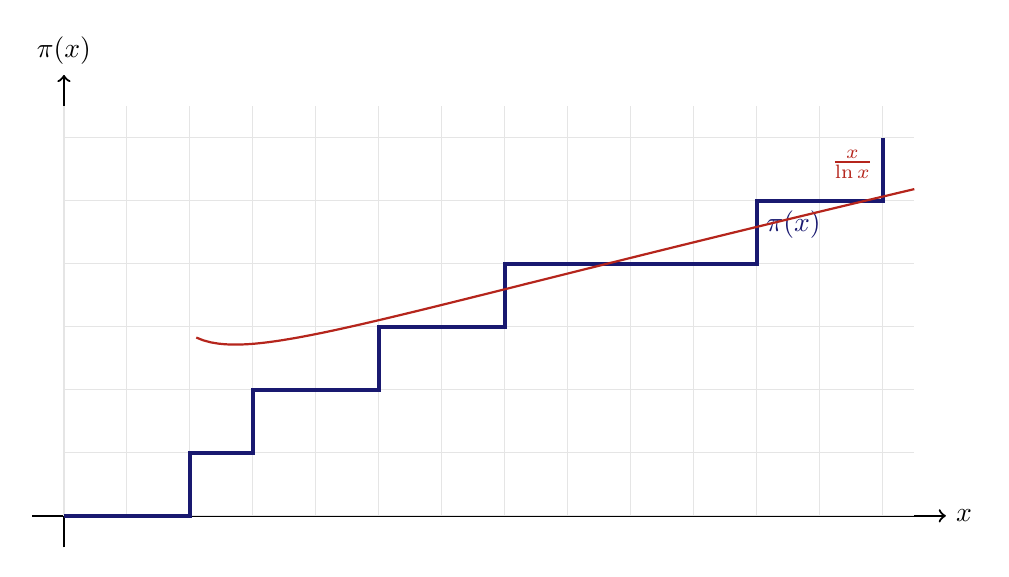
\begin{tikzpicture}[scale=0.8]
    % Achsen
    \draw[->, thick] (-0.5,0) -- (14,0) node[right] {$x$};
    \draw[->, thick] (0,-0.5) -- (0,7) node[above] {$\pi(x)$};
    
    % Gitter (leicht)
    \draw[gray!20, step=1cm] (0,0) grid (13.5,6.5);

    % Treppenfunktion pi(x)
    \draw[ultra thick, MidnightBlue] (0,0) -- (2,0) -- (2,1) -- (3,1) -- (3,2) -- (5,2) -- (5,3) -- (7,3) -- (7,4) -- (11,4) -- (11,5) -- (13,5) -- (13,6);
    \node[MidnightBlue, below right] at (11, 5) {$\pi(x)$};

    % Asymptotische Kurve x/ln(x)
    \draw[thick, BrickRed, domain=2.1:13.5, samples=100] plot (\x, {\x/ln(\x)});
    \node[BrickRed, above left] at (13, 5.2) {$\frac{x}{\ln x}$};
\end{tikzpicture}
\end{center}
\end{math-stroke}

\begin{math-stroke}[Asymptotische Verteilung der Primzahlen]
\begin{theorem}[Primzahlsatz]\label[theorem]{thm:primzahlsatz}
Die Primzahlfunktion $\pi(x)$ verhält sich asymptotisch wie die Funktion $\frac{x}{\ln x}$:
\begin{equation}\label{eq:primzahlsatz}
\pi(x) \sim \frac{x}{\ln x} \iff \lim_{x \to \infty} \frac{\pi(x)}{\frac{x}{\ln x}} = 1.
\end{equation}
\end{theorem}

\begin{explanation-of-steps}
Die Notation $f(x) \sim g(x)$ bedeutet, dass der Quotient der beiden Funktionen für $x \to \infty$ gegen $1$ konvergiert. Dies gibt uns eine präzise Aussage über die \qt{Dichte} der Primzahlen: In der Nähe einer großen Zahl $x$ ist etwa jede $\ln x$-te Zahl eine Primzahl.
\end{explanation-of-steps}
\end{math-stroke}

\subsection{Eulersche Phi-Funktion und Kongruenzen}

\begin{spoken-clean}[01:11:00 - 01:21:44]
Ein weiteres wichtiges Konzept ist die Eulersche $\varphi$-Funktion. Sie gibt an, wie viele Zahlen kleiner oder gleich $n$ zu $n$ teilerfremd sind, also einen $\operatorname{ggT}$ von $1$ mit $n$ haben. Für eine Primzahl $p$ ist das besonders einfach: Da alle Zahlen kleiner als $p$ teilerfremd zu $p$ sind, gilt einfach $\varphi(p) = p - 1$.

Das führt uns schließlich zum Begriff der Kongruenz modulo $n$. Wir sagen, zwei ganze Zahlen $a$ und $b$ sind kongruent modulo $n$, wenn ihre Differenz durch $n$ teilbar ist. Das ist die mathematische Formulierung für das Rechnen mit Resten, wie wir es von der Uhrzeit kennen. Diese Relation ist eine Äquivalenzrelation, und die Äquivalenzklassen nennen wir Restklassen. Das Schöne ist, dass diese Kongruenz mit der Addition und Multiplikation verträglich ist, was uns erlaubt, in diesen Restklassen ganz normal zu rechnen. Das werden wir nächste Woche noch genauer vertiefen. Vielen Dank für heute und bis zum nächsten Mal!
\end{spoken-clean}

\begin{math-stroke}[Die Eulersche $\varphi$-Funktion]
\begin{definition}[Eulersche $\varphi$-Funktion]\label[definition]{def:euler-phi}
Die \newterm{Eulersche $\varphi$-Funktion} (auch Totient-Funktion) $\varphi \colon \mathbb{N} \setminus \{0\} \to \mathbb{N}$ ordnet jeder Zahl $n$ die Anzahl der zu $n$ teilerfremden natürlichen Zahlen im Bereich $1 \le a \le n$ zu:
\[
\varphi(n) := \bigl| \{ a \in \mathbb{N} \mid 1 \le a \le n \land \operatorname{ggT}(a, n) = 1 \} \bigr|.
\]
\end{definition}

\begin{examples}
\begin{itemize}
    \item \textbf{$\varphi(1) = 1$} (da $\operatorname{ggT}(1, 1) = 1$).
    \item \textbf{$\varphi(2) = 1$} (nur $a=1$).
    \item \textbf{$\varphi(3) = 2$} ($a=1, 2$).
    \item \textbf{$\varphi(4) = 2$} ($a=1, 3$).
    \item \textbf{$\varphi(6) = 2$} ($a=1, 5$).
    \item \textbf{Für Primzahlen $p$:} $\varphi(p) = p - 1$.
\end{itemize}
\end{examples}
\end{math-stroke}

\begin{math-stroke}[Kongruenz modulo $n$]
\begin{definition}[Kongruenz]\label[definition]{def:kongruenz}
Sei $n \in \mathbb{N} \setminus \{0\}$. Zwei Zahlen $a, b \in \mathbb{Z}$ heißen \newterm{kongruent modulo $n$}, falls $n$ ihre Differenz teilt:
\[
a \equiv b \pmod n :\iff n \mid (a - b).
\]
Die Äquivalenzklasse von $a$ wird als \newterm{Restklasse} bezeichnet und mit $\bar{a}$ oder $[a]_n$ notiert:
\[
\bar{a} := \{ x \in \mathbb{Z} \mid x \equiv a \pmod n \}.
\]
\end{definition}

\begin{proposition}[Verträglichkeit mit Grundrechenarten]\label[proposition]{prop:kongruenz-vertraeglichkeit}
Seien $a \equiv a' \pmod n$ und $b \equiv b' \pmod n$. Dann gilt:
\begin{enumerate}[label=\textbf{(\roman*)}]
    \item $a + b \equiv a' + b' \pmod n$
    \item $a \cdot b \equiv a' \cdot b' \pmod n$
\end{enumerate}
\end{proposition}
\end{math-stroke}

\begin{proof}[Beweis von Proposition \ref{prop:kongruenz-vertraeglichkeit}]
\begin{math-stroke}[Beweis der Verträglichkeit]
\begin{short-proof}[Beweis der Verträglichkeit]
Nach Voraussetzung gilt $a - a' = k \cdot n$ und $b - b' = \ell \cdot n$ für $k, \ell \in \mathbb{Z}$.
\begin{itemize}
    \item \textbf{Addition:} $(a + b) - (a' + b') = (a - a') + (b - b') = (k + \ell) \cdot n \equiv 0 \pmod n$.
    \item \textbf{Multiplikation:} $ab - a'b' = ab - a'b + a'b - a'b' = (a - a')b + a'(b - b') = (kb + a'\ell) \cdot n \equiv 0 \pmod n$.
\end{itemize}
\end{short-proof}
\end{math-stroke}
\end{proof}

\begin{nice-box}[Zusammenfassung der Schlüsselkonzepte]
In dieser Vorlesung haben wir die Grundlagen der elementaren Zahlentheorie erarbeitet:
\begin{itemize}
    \item \textbf{Division mit Rest:} Für $a \in \mathbb{N} \setminus \{0\}$ und $b \in \mathbb{Z}$ existieren eindeutige $q, r \in \mathbb{Z}$ mit $b = aq + r$ und $0 \le r < a$.
    \item \textbf{Größter gemeinsamer Teiler (ggT):} Der $\operatorname{ggT}(a, b)$ ist der eindeutige positive gemeinsame Teiler, der von jedem anderen gemeinsamen Teiler geteilt wird. Er lässt sich als Linearkombination darstellen (Bézout-Identität: $\operatorname{ggT}(a, b) = ax + by$).
    \item \textbf{Euklidischer Algorithmus:} Ein hocheffizientes Verfahren zur Berechnung des $\operatorname{ggT}$ durch sukzessive Division mit Rest.
    \item \textbf{Fundamentalsatz der Arithmetik:} Jede ganze Zahl ungleich null besitzt eine bis auf die Reihenfolge eindeutige Primfaktorzerlegung.
    \item \textbf{Satz von Euklid:} Es existieren unendlich viele Primzahlen.
    \item \textbf{Kongruenz modulo $n$:} Eine Äquivalenzrelation auf $\mathbb{Z}$, die mit der Addition und Multiplikation verträglich ist und das Fundament der modularen Arithmetik bildet.
\end{itemize}
\end{nice-box}

\begin{ai-global-state-checkpoint-invisible-content}
% timestamp: 01:21:44
% topic: Einführung der Eulerschen Phi-Funktion und der Kongruenzrechnung.
% board_state: def:euler-phi, def:kongruenz, prop:kongruenz-vertraeglichkeit.
% next_goal: Vertiefung der Restklassenringe in der nächsten Woche.
% open_loops: Schubfachprinzip auf dem Aufgabenblatt.
\end{ai-global-state-checkpoint-invisible-content}

% [SYSTEM] Refinement complete